\begin{figure*}[t]
  \centering
  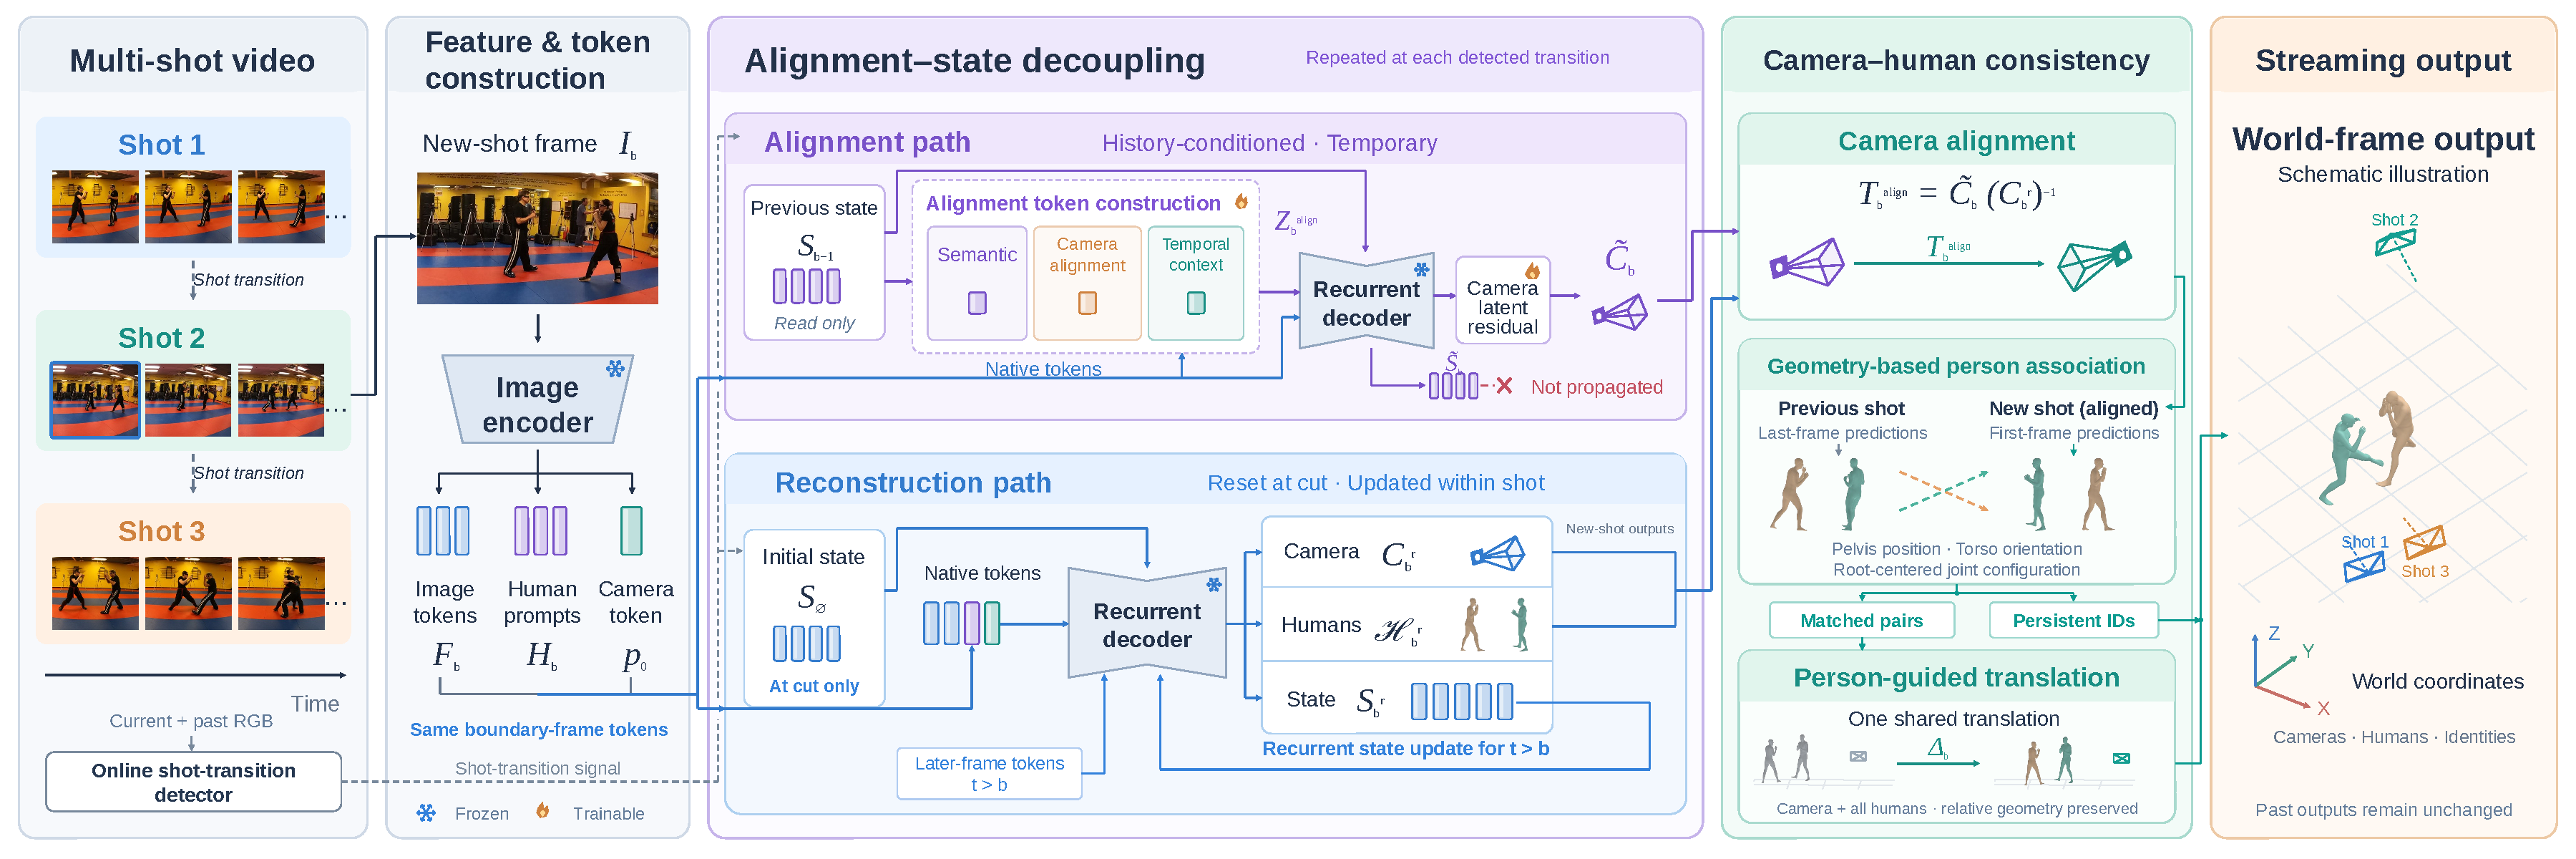
\includegraphics[width=\textwidth]{figures/method.pdf}
  % 中文图注：Shot3R 方法概览。历史条件路径临时推断镜头间关系，只有重新初始化路径传播递归状态。
  % 基于几何的人物关联延续人物身份，共享变换将新镜头输出置于统一世界坐标系。最右侧面板为示意图。
  % 图内标签中文：Monocular stream=单目视频流；Input representations=输入表示；
  % Decoupling alignment from state propagation=将对齐与状态传播解耦；
  % Alignment path / temporary=对齐路径／临时使用；Reconstruction path / propagated=重建路径／持续传播；
  % Camera and human consistency=相机与人体一致性；World-frame output=世界坐标系输出；
  % Schematic illustration=示意图；Streaming output=流式输出。
  % 其余图内标签中文：previous/new shot=前一／新镜头；shot transition=镜头切换；Online detector=在线检测器；
  % current and past RGB only=仅当前与历史 RGB；Previous state=先前状态；Typed alignment tokens=带类型的对齐 token；
  % Backbone input tokens / Backbone tokens=主干输入 token／主干 token；Temporal context=时间上下文；
  % Used only for alignment=仅用于对齐；Inter-shot camera alignment=镜头间相机对齐；
  % Camera latent residual=相机潜变量残差；Geometry-based person association=基于几何的人物关联；
  % Shared transform for cameras and humans=相机与人体共享变换；Shared world-frame transform=共享世界坐标变换；
  % New-shot outputs=新镜头输出；Subsequent frames=后续帧；Temporary alignment vs. propagated state=临时对齐与持续传播的状态。
  % 输出面板为示意性世界坐标布局，不代表模型输出的直接渲染。
  \caption{Overview of \method{}. The history-conditioned path temporarily
  infers the inter-shot relation, while only the reinitialized path propagates
  recurrent state. Geometry-based association transfers identities, and a
  shared transform places new-shot outputs in the common world frame. The
  rightmost panel is schematic.}
  \label{fig:method}
\end{figure*}
